% !TEX root = ../main.tex

\chapter{Outroduction}
\label{ch:observations}

\startcontents[chapters]

\vfill

\begin{alltt}\sffamily
Yet my state is well,
is to take those things for bird,
and God keep him out of my sight,
I do spy some marks of love in her.

With catlike watch,
I have watch'd and travell'd hard,
and some will mourn in ashes,
so that hardly can I check my eyes from tears.

Pillars of the state,
word out of his right sense,
first emperor of Rome Mark Anthony.

Have you had quiet guard,
though art a guard too wanton for the head,
of each other's watch.
\end{alltt}

\newpage
\minicontents
\spirals


The research presented in this thesis described \acf{AMC} and its evaluation. The first part of this knowledge was embodied in an artefact \url{pata.physics.wtf} and the second part was formulated as a theoretical framework to help interpretation of products of \ac{AMC}.

The overall research methodology was described in the \nameref{ch:methodology} chapter\marginpar{§~\ref{ch:methodology}} but it can be summarised having a subjective, transdisciplinary approach, using creative computing, experimental and exploratory methodologies. Specifically, existing literature was synthesised\marginpar{\textspiral~\ref{p:lit}}, algorithms were designed, an artefact was created using iterative exploratory development\marginpar{\textspiral~\ref{p:practice}}, a theoretical framework was developed \marginpar{\textspiral~\ref{p:theory}} and the project contained a critical reflection and analysis of the artefact presented\marginpar{\textspiral~\ref{p:analysis}}. 


\section{Observations}

The artefact \url{pata.physics.wtf} should be seen as an artwork inspired by and dedicated to \ac{AMC}, pataphysics, \ac{OULIPO} and programming culture.

On the face of it this thesis might appear to argue that computers can be seen as creative entities. This is however not the case. In fact I argue against this in the \nameref{ch:interpretation}\marginpar{§~\ref{ch:interpretation}} chapter---the computer is always only a tool for a human's creativity and nothing more. This is not to say that a computer can't be `taught' creative techniques, which is what I have called \ac{AMC}.

% Some of the issues highlighted in the \nameref{ch:introduction}\marginpar{§~\ref{ch:introduction}} were described in terms of pataphysical antinomies. 

% \begin{itemize}
%   \item Polymorphism (generalisation) opposes particularity.
%   \item Precision opposes exceptions and contradictions.
%   \item Logic and structure oppose the imaginary and paradox.
%   \item Cross-compatibility opposes the mutually exclusive.
%   \item Responsiveness opposes the specific.
%   \item Relevance opposes the creative.
% \end{itemize}

Figure~\ref{fig:patarc2} shows an abstract view of \url{pata.physics.wtf}\marginpar{\faicon{object-group}~\ref{fig:patarc2}}.

\begin{figure}[!htbp]
  \centering
  \begin{tikzpicture}[node distance = 1.5cm and 2.5cm]
    \spiral[]{center={(4.5,-2.3)}, end angle=45, end radius= 0.3, revolutions=4};
    \node [box] (corpus) {Corpus};
    \node [box, below = of corpus] (index) {Index};
    \node [box, right = of index] (pata) {};
    \node [box, above = of pata] (user) {User};
    \draw [sa] (corpus) -- node [left] {setup} (index);
    \draw [sa] (user) -- node [right] {query} (pata);
    \draw [sa] (pata) -- node [below] {patadata} (index);
    \draw [sa] (index) -- node [above = 10pt] {results} (user);
  \end{tikzpicture}
  \caption[Pataphysical system architecture (again)]{Pataphysical system architecture (again)}
  \label{fig:patarc2}
\end{figure}


\section{Answers}
\label{s:answers}

In the introduction\marginpar{§~\ref{ch:introduction}} I asked several questions that I attempted to answer with the research presented in this thesis. This section contains brief answers from 50.000 feet\footnote{Inspired by Tim Berners-Lee's articles on the web in its early days \autocite*{TBL1998}.}, meaning they provide a top-down view of the answer and pointers to where in the thesis readers can find more elaborations.

\paragraph{What is the relationship between pataphysics and creativity?}

The \nameref{ch:foundations}\marginpar{§~\ref{ch:foundations}} chapter discusses this in detail. Pataphysics provides many philosophical principles which can be turned into creative techniques and constraints. In specific table~\ref{tab:creatpata}\marginpar{\faicon{table}~\ref{tab:creatpata}} shows the similarities and differences between pataphysics and creativity. One of the key attributes of creativity for example is the idea of bisociation---the juxtaposition of the dissimilar---which relates directly to the pataphysical concept of the antinomy\marginpar{§~\ref{s:antinomy}}---the simultaneous existence of the mutually exclusive.

\paragraph{How is computer creativity related to artificial intelligence?}

Much of the research in computational creativity (see chapter~\ref{s:compcrea}\marginpar{§~\ref{s:compcrea}}) stems from the area of \ac{AI}. In the \nameref{s:theoryanalysis} chapter\marginpar{§~\ref{s:theoryanalysis}} I mentioned the similarities in these two fields. In particular, I discussed the ideas of free will and surprise, understanding and simulation, and brains and computers.

\paragraph{Should we distinguish between computationally automated or emulated creative processes and the programmer's input?}

Yes. Just like the process and product are both equally important, the computational process and the programmer are both essential. This is discussed in the chapter\marginpar{§~\ref{s:programmer}} on \nameref{s:programmer} but also gets addressed in the \nameref{s:o-i} section in chapter~\ref{ch:evaluation}\marginpar{§~\ref{s:o-i}} on \nameref{ch:evaluation}.

\paragraph{How can a machine's creative output be evaluated?}

Previous attempts at evaluating computer creativity are critically reviewed in chapter~\ref{s:creattributes}\marginpar{§~\ref{s:creattributes}}. The \nameref{s:creatint} chapter\marginpar{§~\ref{s:creatint}} then introduces one of the main original contributions of this research: a new framework for the evaluation and interpretation of creative artefacts (this can be applied to human-made and machine-made products). Since the perception of creativity is subjective it cannot be quantified in objective terms. By providing a framework that takes into account all possible contextually relevant contributors though we can approximate an objective evaluation.

\paragraph{How can information retrieval be infused with creativity?}

This is explored in chapter~\ref{s:pataputers}\marginpar{§~\ref{s:pataputers}} and of course the \nameref{ch:implementation} chapter, where the development of \url{pata.physics.wtf} is explained\marginpar{§~\ref{ch:implementation}}. This is a direct example of creative exploratory \ac{IR}.


\section{Contributions}

The original contributions to knowledge presented by this doctoral research can be broken down into the 4 points below.

\begin{itemize}
  \item Three pataphysical search algorithms (clinamen, syzygy and antinomy).
  \item A creative exploratory search tool demonstrating the \ac{AMC}.
  \item 7 subjective criteria and 5 objective constraints for defining creativity.
  \item A combined framework for evaluating and interpreting creativity.
\end{itemize}


\section{And Finally}

\emph{Pataphysics is the science\ldots}


\section{From the Outroduction to Paris by Sea}

\begin{figure}[!htb]
\centering
  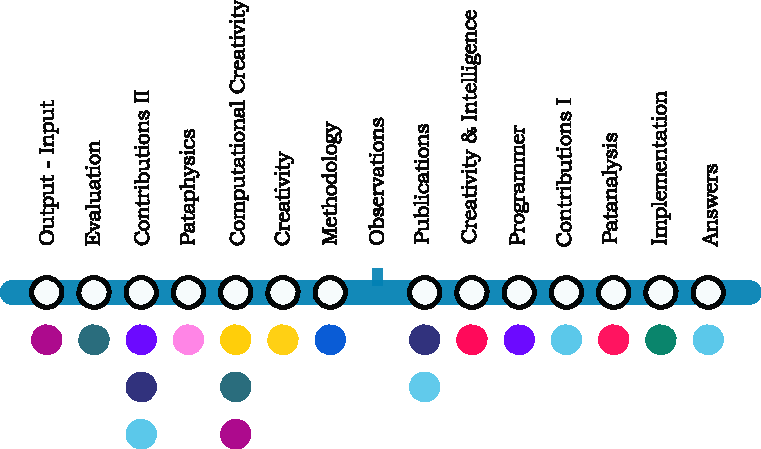
\includegraphics{outro.pdf}
\end{figure}

The conclusion chapter \outro~ ties together all other chapters (specifically \found, \inter, and \imple) but perhaps mainly provides the answers for the research questions posed in the \nameref{ch:introduction} \intro.

\begin{figure}[!htb]
\centering
  
\includegraphics[width=\textwidth]{legend.pdf}
\end{figure}

\stopcontents[chapters]
